\section{SEP 2019}  

\subsection{Cache Performance Analysis}

\begin{KR}{Cache Hit Rate Calculation}
    \paragraph{Given information analysis}
    \begin{itemize}
        \item Identify data type size (e.g., int = 4 bytes on 32-bit system)
        \item Note cache line size (e.g., 64 bytes)
        \item Determine access pattern (sequential vs. random)
    \end{itemize}
    
    \paragraph{Calculate elements per cache line}
    \begin{itemize}
        \item Elements per line = Cache line size / Element size
        \item For sequential access: First access = miss, rest = hits
        \item Hit rate = (Elements per line - 1) / Elements per line
    \end{itemize}
    
    \paragraph{Apply formula}
    \begin{itemize}
        \item Hit rate = Number of hits / Total accesses
        \item Express as percentage or decimal
    \end{itemize}
\end{KR}

\begin{example2}{Cache Access Analysis}
    Given code accessing an integer array sequentially:
    
\begin{lstlisting}[language=C, style=basesmol]
#define N (10*1000*1000)
int arVL[N];
for (int i = 0; i < N; i++) {
    sum += arVL[i];
}
\end{lstlisting}

    \tcblower
    
    \textbf{Analysis:}
    \begin{itemize}
        \item 32-bit system: int = 4 bytes
        \item Cache line size: 64 bytes
        \item Elements per cache line: 64/4 = 16 integers
        \item Access pattern: Sequential
        \item For every 16 accesses: 1 miss + 15 hits
        \item Hit rate: 15/16 = 0.9375 = 93.75\%
    \end{itemize}
\end{example2}

\begin{KR}{Average Memory Access Time}
    \paragraph{Multi-level cache formula}
    \begin{itemize}
        \item $T_a = T_1 + (1-h_1) \times [T_2 + (1-h_2) \times [T_3 + (1-h_3) \times T_{mem}]]$
        \item Where $T_i$ = access time for level i, $h_i$ = hit rate for level i
    \end{itemize}
    
    \paragraph{Step-by-step calculation}
    \begin{itemize}
        \item Convert clock cycles to nanoseconds: cycles $\times$ cycle time
        \item Apply formula from innermost level outward
        \item L3 miss probability = $(1-h_1) \times (1-h_2) \times (1-h_3)$
    \end{itemize}
\end{KR}

\begin{example2}{Memory Access Time Calculation}
    2 GHz processor (0.5 ns cycle), 90\% hit rate on all levels:
    
    \begin{tabular}{|l|l|}
        \hline
        L1 Cache & 4 cycles = 2.0 ns \\
        L2 Cache & 10 cycles = 5.0 ns \\
        L3 Cache & 40 cycles = 20.0 ns \\
        Main Memory & 60 ns \\
        \hline
    \end{tabular}
    
    \tcblower
    
    \textbf{Calculation:}
    \begin{itemize}
        \item $T_a = 2.0 + 0.1 \times [5.0 + 0.1 \times [20.0 + 0.1 \times 60.0]]$
        \item $T_a = 2.0 + 0.1 \times [5.0 + 0.1 \times [20.0 + 6.0]]$
        \item $T_a = 2.0 + 0.1 \times [5.0 + 0.1 \times 26.0]$
        \item $T_a = 2.0 + 0.1 \times [5.0 + 2.6] = 2.0 + 0.1 \times 7.6$
        \item $T_a = 2.0 + 0.76 = 2.76$ ns
    \end{itemize}
\end{example2}

\subsection{Build System Analysis}

\begin{KR}{Make Dependency Analysis}
    \paragraph{Examine file timestamps}
    \begin{itemize}
        \item List all source files (.c) and object files (.o)
        \item Compare timestamps: source newer than object = recompile needed
        \item Check dependency requirements in Makefile
    \end{itemize}
    
    \paragraph{Apply make rules}
    \begin{itemize}
        \item Target depends on all listed prerequisites
        \item Suffix rule (.c.o:) applies to C source compilation
        \item Variable substitution: \$@ = target name, \$< = first prerequisite
    \end{itemize}
    
    \paragraph{Determine final executable name}
    \begin{itemize}
        \item Follow target name and any modifications (e.g., \$@.e)
        \item Check for explicit output naming in link command
    \end{itemize}
\end{KR}

\begin{example2}{Make Analysis}
    Given Makefile and file listing:
    
\begin{lstlisting}[language=bash, style=basesmol]
# Makefile
CFL = -g
CMP = gcc $(CFL)
app: main1.o mythread.o scheduler.o queues.o mylist.o
    $(CMP) main1.o mythread.o scheduler.o queues.o mylist.o -o $@.e
.c.o:
    $(CMP) -c $<

# File listing (key timestamps)
# mylist.c    Feb 24 09:31  (source)
# mylist.o    Feb 24 09:21  (object)
# queues.c    Feb 24 09:25  (source)  
# queues.o    Feb 24 09:21  (object)
\end{lstlisting}

    \tcblower
    
    \textbf{Analysis:}
    \begin{itemize}
        \item Files to recompile: mylist.c and queues.c (sources newer than objects)
        \item Final executable: app.e (from target "app" + ".e" extension)
        \item Other .o files are up-to-date, no recompilation needed
    \end{itemize}
\end{example2}

\raggedcolumns
\columnbreak

\subsection{Process Creation}

\begin{KR}{Fork Analysis}
    \important{SAME GRAPHIC AS IN SEP07}
    \paragraph{Draw process tree}
    \begin{itemize}
        \item Start with original process
        \item At each fork(), branch into parent and child
        \item Label each process with execution path
    \end{itemize}
    
    \paragraph{Trace execution paths}
    \begin{itemize}
        \item Parent: fork() returns child PID (> 0)
        \item Child: fork() returns 0
        \item Follow if-else logic for each process
    \end{itemize}
    
    \paragraph{Count results}
    \begin{itemize}
        \item Total processes = original + all children created
        \item Count specific outputs by tracing paths to printf statements
    \end{itemize}
\end{KR}

\begin{example2}{Process Creation Analysis}
    Analyze the following code:
    
\begin{lstlisting}[language=C, style=basesmol]
if (fork() > 0)
    fork();
else {
    fork();
    if (fork() > 0)
        printf("Hello World\n");
}
\end{lstlisting}

    \tcblower
    
    \textbf{Process tree and analysis:}
    \begin{itemize}
        \item Original process P forks $\rightarrow$ creates child C1
        \item Parent P (fork() > 0): executes second fork() $\rightarrow$ creates child C2
        \item Child C1 (fork() == 0): executes fork() $\rightarrow$ creates child C3
        \item Child C1: executes second fork() $\rightarrow$ creates child C4, then prints
        \item Child C3: executes second fork() $\rightarrow$ creates child C5, then prints
    \end{itemize}
    
    \textbf{Results:}
    \begin{itemize}
        \item Additional processes created: 5 (C1, C2, C3, C4, C5)
        \item "Hello World" printed: 2 times (by C1 and C3)
    \end{itemize}
\end{example2}

\subsection{Memory Management}

\begin{KR}{Buddy System Fragmentation}
    \paragraph{Determine buddy block sizes}
    \begin{itemize}
        \item For each allocation request, find smallest power-of-2 block that fits
        \item Block size = $2^{\lceil \log_2(\text{request size}) \rceil}$
    \end{itemize}
    
    \paragraph{Calculate internal fragmentation}
    \begin{itemize}
        \item Fragmentation per block = Block size - Requested size
        \item Total fragmentation = Sum of all individual fragmentations
    \end{itemize}
    
    \paragraph{Account for merging}
    \begin{itemize}
        \item When blocks are freed, buddies may merge
        \item Track which blocks remain allocated vs. freed
    \end{itemize}
\end{KR}

\begin{example2}{Buddy System Analysis}
    8MB system allocates buffers: 62KB, 34KB, 9KB
    
    \tcblower
    
    \textbf{Allocation analysis:}
    \begin{itemize}
        \item \textcolor{orange}{62KB} $\rightarrow$ 64KB block (internal fragmentation: 2KB)
        \item \textcolor{blue}{34KB} $\rightarrow$ 64KB block (internal fragmentation: 30KB)
        \item \textcolor{frog}{9KB} $\rightarrow$ 16KB block (internal fragmentation: 7KB)
        \item Total internal fragmentation: 2 + 30 + 7 = 39KB
    \end{itemize}

    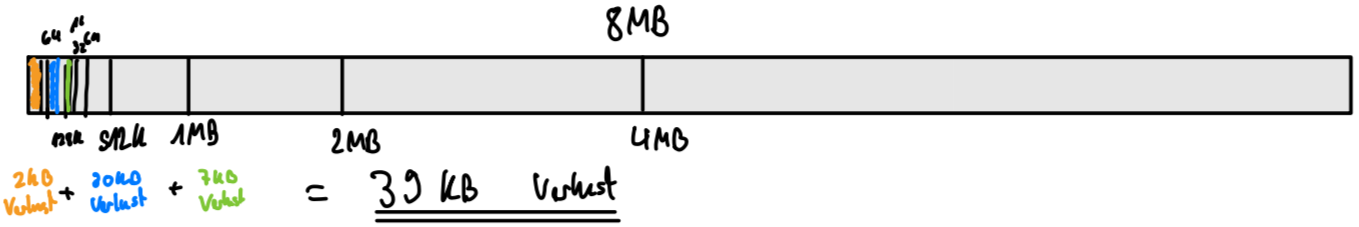
\includegraphics[width=\linewidth]{BUDDYSYSTEM_SEP19.png}
    
    The remaining memory is still available for allocation but in specific block sizes according to the buddy system structure.
\end{example2}

\begin{KR}{Page Table Calculations}
    \paragraph{Extract address components}
    \begin{itemize}
        \item Page Directory bits determine max number of page tables
        \item Page Number bits determine entries per page table
        \item Offset bits determine page size: $2^{\text{offset bits}}$
    \end{itemize}
    
    \paragraph{Calculate system limits}
    \begin{itemize}
        \item Page size = $2^{\text{offset bits}}$ bytes
        \item Max page tables = $2^{\text{directory bits}}$
        \item Entries per page table = $2^{\text{page number bits}}$
        \item Max frames = Max page tables $\times$ Entries per table
    \end{itemize}
\end{KR}

\begin{example2}{Page Table Structure Analysis}
    32-bit addresses with 6-bit page directory, 8-bit page number, 10-bit offset:
    
    \tcblower
    
    \textbf{Calculations:}
    \begin{itemize}
        \item Page size: $2^{10}$ = 1024 bytes = 1KB
        \item Page directory entries: $2^6$ = 64 page tables max
        \item Entries per page table: $2^8$ = 256 pages per table
        \item Each page table entry: 4 bytes (32-bit system)
        \item Page directory size: 64 entries $\times$ 4 bytes = 256 bytes
        \item Max system frames: 64 $\times$ 256 = 16,384 frames
    \end{itemize}
\end{example2}

\subsection{Page Replacement}

\begin{KR}{LRU Page Replacement}
    \paragraph{Track page access order}
    \begin{itemize}
        \item Maintain timestamp or access order for each page in memory
        \item On page fault, identify least recently used page
        \item Replace LRU page with new page
    \end{itemize}
    
    \paragraph{Handle page faults}
    \begin{itemize}
        \item Mark page fault when referenced page not in memory
        \item Load new page into frame of LRU page
        \item Update access timestamps for all affected pages
    \end{itemize}
    
    \paragraph{Apply demand paging}
    \begin{itemize}
        \item First access to any page is compulsory miss
        \item Subsequent accesses depend on memory capacity and access pattern
    \end{itemize}
\end{KR}

\begin{example2}{LRU Page Replacement Trace}
    \important{SAME EXERCISE AGAIN}
    Process references pages: 8,7,5,8,7,3,5,1,3,4,2,1,8,3,1,2
    
    4 frames available, initially empty:
    
    \begin{tabular}{|c|c|c|c|c|c|c|c|c|c|c|c|c|c|c|c|c|}
        \hline
        Reference & 8 & 7 & 5 & 8 & 7 & 3 & 5 & 1 & 3 & 4 & 2 & 1 & 8 & 3 & 1 & 2 \\
        \hline
        Frame 1 & 8 & 8 & 8 & 8 & 8 & 8 & 8 & 1 & 1 & 1 & 1 & 1 & 1 & 1 & 1 & 1 \\
        Frame 2 &  & 7 & 7 & 7 & 7 & 7 & 7 & 7 & 4 & 4 & 4 & 3 & 3 & 3 & 3 & 3 \\
        Frame 3 &  &  & 5 & 5 & 5 & 5 & 5 & 5 & 5 & 2 & 2 & 2 & 2 & 2 & 2 & 2 \\
        Frame 4 &  &  &  &  &  & 3 & 3 & 3 & 3 & 3 & 8 & 8 & 8 & 8 & 8 & 8 \\
        \hline
        Page Fault & X & X & X &  &  & X &  & X &  & X & X &  &  &  &  &  \\
        \hline
    \end{tabular}
    
    \tcblower
    
    \textbf{Total page faults: 8}
    
    Key LRU decisions:
    \begin{itemize}
        \item At time 8: Page 1 replaces page 8 (LRU)
        \item At time 10: Page 4 replaces page 7 (LRU) 
        \item At time 11: Page 2 replaces page 5 (LRU)
        \item At time 13: Page 8 replaces page 3 (LRU)
    \end{itemize}

    \textbf{Least recently used} (Linux Approach):\\
    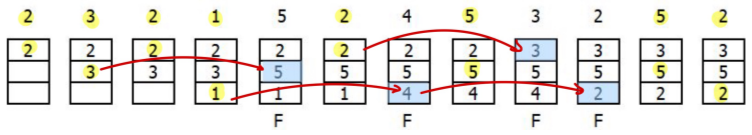
\includegraphics[width=0.5\linewidth]{page_replacement_SEP19.png}
\end{example2}

\subsection{Real-Time Scheduling}

\begin{KR}{Earliest Deadline First (EDF)}
    \paragraph{Calculate absolute deadlines}
    \begin{itemize}
        \item For each task instance: Deadline = Arrival time + Period
        \item Track all active tasks (arrived but not completed)
        \item Update deadlines when new instances arrive
    \end{itemize}
    
    \paragraph{Schedule by earliest deadline}
    \begin{itemize}
        \item At each scheduling point, select task with earliest absolute deadline
        \item Preempt running task if new arrival has earlier deadline
        \item Use period as tiebreaker for equal deadlines (shorter period wins)
    \end{itemize}
    
    \paragraph{Handle rescheduling points}
    \begin{itemize}
        \item Reschedule when task completes or suspends
        \item Reschedule at fixed intervals if specified
        \item Reschedule when new task arrives (if preemptive)
    \end{itemize}
\end{KR}

\begin{example2}{EDF Scheduling}
    Three periodic tasks with rescheduling every 4ms or when a task is suspended: 
    
    \begin{tabular}{|c|c|c|}
        \hline
        Task & Period & Execution Time \\
        \hline
        \textcolor{red}{T1} & 4ms & 1ms \\
        \textcolor{red}{T2} & 8ms & 4ms \\
        \textcolor{red}{T3} & 12ms & 3ms \\
        \hline
    \end{tabular}

    Priority: in case of equal deadlines, shorter period wins.

    \tcblower
    \textbf{Preemptive Diagram:}\\
    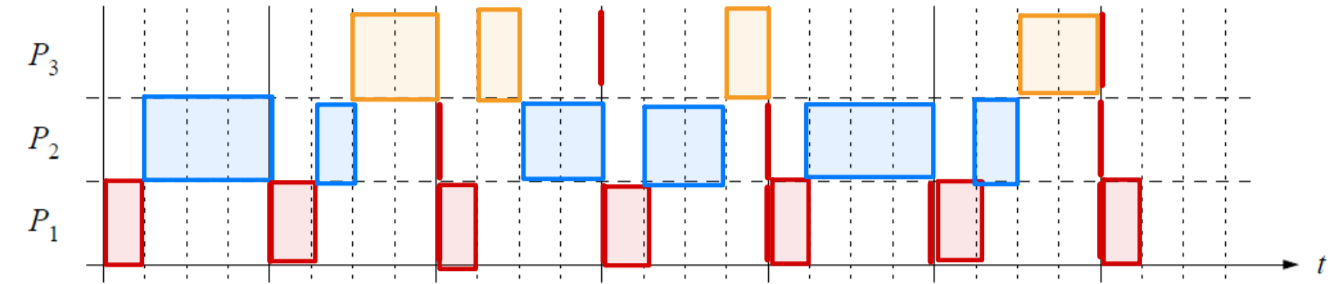
\includegraphics[width=\linewidth]{scheduling_diagram_SEP19.png}
    \vspace{2mm}\\
    \textbf{Timeline analysis (first 24ms):}
    \begin{itemize}
        \item t=0: T1(dl=4), T2(dl=8), T3(dl=12) arrive $\rightarrow$ Schedule T1
        \item t=1: T1 completes $\rightarrow$ Schedule T2  
        \item t=4: T1(dl=8) arrives, T2 continues (dl=8, but T2 started first)
        \item t=5: T1 executes (same deadline, shorter period wins)
        \item t=6: T1 completes $\rightarrow$ Schedule T2
        \item t=8: T1(dl=12), T2(dl=16) arrive, T3 continues
        \item And so on...
    \end{itemize}
    
    The schedule ensures all deadlines are met with this task set.
\end{example2}

\begin{example2}{General Scheduling Example}\\
    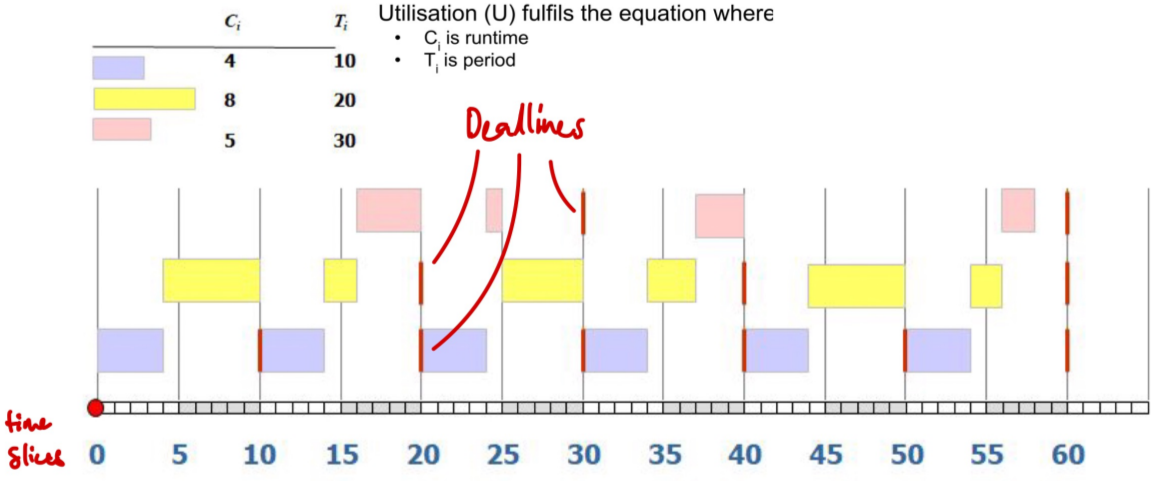
\includegraphics[width=\linewidth]{general_scheduling_example.png}
\end{example2}

\subsection{Multi-Level Scheduling}

\begin{KR}{Priority-Based Multi-Level Scheduling}
    \paragraph{Organize by priority levels}
    \begin{itemize}
        \item Group processes by priority (higher number = higher priority)
        \item Maintain separate ready queue for each priority level
        \item Always schedule from highest priority non-empty queue
    \end{itemize}
    
    \paragraph{Apply Round Robin within priority}
    \begin{itemize}
        \item Use time quantum for processes at same priority level
        \item Move process to end of same priority queue when quantum expires
        \item New arrivals join appropriate priority queue
    \end{itemize}
    
    \paragraph{Handle preemption}
    \begin{itemize}
        \item Higher priority process always preempts lower priority
        \item Preemption occurs immediately when higher priority task arrives
        \item Preempted task returns to head of its priority queue
    \end{itemize}
\end{KR}

\begin{example2}{Multi-Level Scheduling with RR}
    Five processes with time quantum = 1:
    
    \begin{tabular}{|c|c|c|c|}
        \hline
        Process & Priority & Arrival & Execution \\
        \hline
        P1 & 0 & 0 & 4 \\
        P2 & 1 & 1 & 3 \\
        P3 & 1 & 2 & 2 \\
        P4 & 0 & 5 & 3 \\
        P5 & 0 & 7 & 2 \\
        \hline
    \end{tabular}
    
    \tcblower

    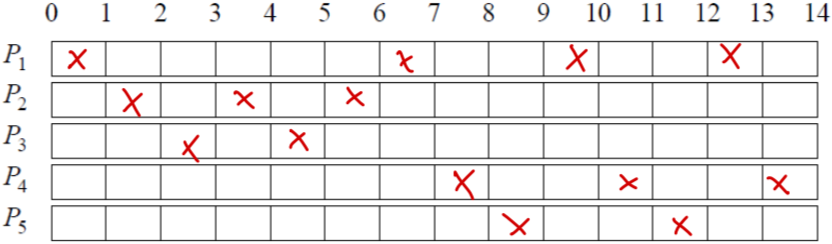
\includegraphics[width=\linewidth]{multilevelsched2.png}
    \vspace{2mm}\\
    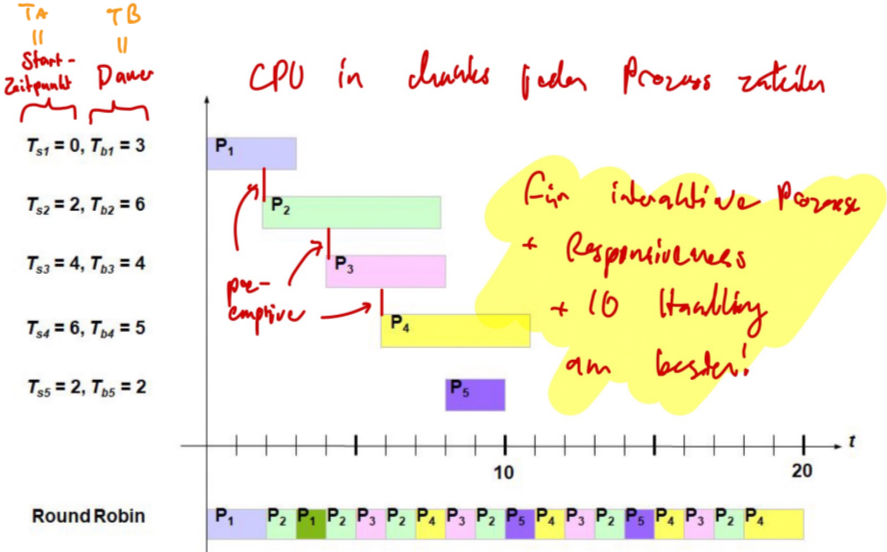
\includegraphics[width=\linewidth]{multilevel_scheduling_SEP19.png}
    \vspace{2mm}\\
    \textbf{Execution timeline:}
    \begin{itemize}
        \item t=0-1: P1 (only process available)
        \item t=1-2: P2 (higher priority, preempts P1)
        \item t=2-3: P3 (same priority as P2, P2's quantum expired)
        \item t=3-4: P2 (continues RR at priority 1)
        \item t=4-5: P3 (completes)
        \item t=5-6: P2 (completes), then P4 starts
        \item t=6-7: P1 (RR at priority 0)
        \item t=7-8: P4 (continues RR), P5 arrives
        \item And so on with RR between P1, P4, P5 at priority 0...
    \end{itemize}
\end{example2}

\subsection{System Concepts}

\begin{KR}{System Call Identification}
    \paragraph{Analyze operation type}
    \begin{itemize}
        \item I/O operations: Screen output, file access, network communication
        \item Resource management: Memory allocation, time delays
        \item Process control: Process creation, inter-process communication
    \end{itemize}
    
    \paragraph{Distinguish user vs kernel operations}
    \begin{itemize}
        \item User mode: Arithmetic, variable manipulation, function calls
        \item Kernel mode: Hardware access, system resource management
        \item Mode switch required for system calls
    \end{itemize}
\end{KR}

\begin{example2}{System Call Requirements}
    Which operations require system calls?
    
    \begin{itemize}
        \item \textcolor{frog}{$\surd$} Screen output (I/O operation)
        \item \textcolor{red}{\textbf{X}} Variable comparison (CPU operation)
        \item \textcolor{frog}{$\surd$} Sleep for 1 second (timer/scheduler)
        \item \textcolor{red}{\textbf{X}} Integer increment (CPU operation)
        \item \textcolor{red}{\textbf{X}} Float increment (CPU operation)
    \end{itemize}
    
    \tcblower
    
    \textbf{Rule of thumb:}
    Operations requiring hardware access, OS services, or resource management need system calls. Pure computational operations do not.
\end{example2}